% !TEX root = ../main/main.tex
\chapter{Reinforcement Learning Framework}
\label{chap:rl}

We articulate the reinforcement-learning (RL) architecture that converts predictive edges into sequential betting policies. Emphasis is placed on safe offline training, interpretability, and integration with classical baselines.

\paragraph{Acronym hygiene.} We spell out acronyms on first use and then keep them concise: off‑policy evaluation (OPE), conservative Q‑learning (CQL), implicit Q‑learning (IQL), TD3 with behavior cloning (TD3+BC) \citep{fujimoto2021td3bc}, and advantage‑weighted actor–critic (AWAC) \citep{nair2020awac}. Where tables list many methods, captions expand names and footnotes include citations.

\section{State of the Art (At a Glance)}
Practical RL for pre-game betting draws on a small set of robust families. We summarize where each fits this problem:
\begin{itemize}
  \item \textbf{Value-based (DQN/Double DQN, Dueling, PER):} discrete actions, data efficiency via replay; good for stake buckets when action spaces are small \citep{mnih2015,vanhasselt2016,wang2016dueling,schaul2016per}.
  \item \textbf{Actor--critic (TRPO/PPO/GAE):} stable on-policy updates with variance reduction; safer promotion when online interaction is allowed (e.g., paper trading) \citep{schulman2015trpo,schulman2016gae,schulman2017ppo}.
  \item \textbf{Deterministic/entropy-regularized control (TD3/SAC):} continuous actions with strong sample efficiency and stability; useful for continuous stake sizing \citep{fujimoto2018td3,haarnoja2018sac}.
  \item \textbf{Distributional critics (C51/QR-DQN/IQN):} model return distributions, often improving stability and calibration of value targets \citep{bellemare2017distributional,dabney2018quantile}.
  \item \textbf{Offline RL (BCQ/BRAC/BEAR/CQL/IQL/TD3+BC):} learn solely from logged data; essential for betting where unsafe exploration is disallowed \citep{fujimoto2019,wu2019brac,kumar2019bear,kumar2020,kostrikov2021iql,agarwal2020offline,levine2020}.
\end{itemize}
For NFL betting we operate primarily in the \emph{offline} regime with conservative promotion gates; when continuous stakes are needed we embed TD3/SAC backbones under offline regularizers, otherwise we use bucketed actions with double/dueling critics and pessimistic objectives.

\subsection*{Why IQL (in practice)}
We use implicit Q-learning (IQL) as the default offline learner because it:
\begin{itemize}
  \item avoids explicit behavior-policy density ratios (robust when logging propensities are noisy),
  \item emphasizes high-advantage actions via expectile regression, reducing extrapolation error,
  \item trains stably with minimal tuning and integrates cleanly with conservative sizing and promotion gates.
\end{itemize}
We compare against CQL and TD3+BC in ablations and promote the most stable model under OPE bounds.

% --- Mathematical reasoning: RL and OPE ---
\section{Foundations: MDPs, Value Functions, and Contractions}\label{sec:bellman-math}
We model betting as a discounted Markov decision process (MDP) $(\mathcal S,\mathcal A, P, r, \gamma)$ where $s\in\mathcal S$ encodes market and team context, $a\in\mathcal A$ encodes a stake decision subject to exposure limits, $P$ governs state transitions across the calendar, $r$ encodes realized log-wealth increments net of frictions, and $\gamma\in(0,1)$ discounts over weeks.
The action-value and state-value functions are
\[
Q^\pi(s,a)=\E\!\left[\sum_{t\ge0}\gamma^t r_{t}\,\middle|\,s_0=s, a_0=a,\pi\right],\quad V^\pi(s)=\E\_{a\sim\pi(\cdot\mid s)}[Q^\pi(s,a)].
\]
The Bellman optimality operator $(\mathcal{T}Q)(s,a)=\E\![r+\gamma\max\_{a'}Q(s',a')\mid s,a]$ is a $\gamma$-contraction in $\|\cdot\|_\infty$, so value iteration converges to $Q^\star$; in practice we stabilize bootstrapping with target networks and replay buffers \citep{sutton2018,mnih2015,vanhasselt2016}.

\section{Off-Policy Evaluation (OPE)}\label{sec:ope}
With behavior $\pi_b$, target $\pi$, and trajectories $\{(s_t,a_t,r_t)\}$, importance ratios
$\rho_t=\pi(a_t\mid s_t)/\pi_b(a_t\mid s_t)$ yield the self-normalized estimator
\[
\hat V_{\text{SNIS}}=\frac{\sum_i \rho_i R_i}{\sum_i \rho_i},\qquad R_i=\sum_t r_{i,t}.
\]
The doubly robust (DR) estimator augments IPS with a learned $Q_{\hat\omega}$:
\[
\hat V_{\text{DR}}=\frac{1}{N}\sum_{i,t}\Big[ Q_{\hat\omega}(s_{i,t},\pi(s_{i,t}))
+ \rho_{i,t}\big(r_{i,t}+\gamma V_{\hat\omega}(s_{i,t+1})-Q_{\hat\omega}(s_{i,t},a_{i,t})\big)\Big],
\]
which is unbiased if either the model or the ratios are correct \citep{dudik2014,jiang2016,thomas2015}.

% Auto-included OPE grid table if present
\IfFileExists{../figures/out/ope_grid_table.tex}{% Auto-generated by py/rl/ope_gate.py
% !TEX root = ../../main/main.tex
\providecommand{\opeGridLabel}{\label{tab:ope-grid}}
\begin{table}[t]
  \centering
  \footnotesize
  \begin{threeparttable}
    \caption[OPE grid (SNIS/DR/ESS)]{Off-policy evaluation grid: SNIS and DR values with effective sample sizes (ESS). Accept=\textbf{Yes}, median DR=0.0226.}
\opeGridLabel
    \setlength{\tabcolsep}{3pt}\renewcommand{\arraystretch}{1.1}
\begin{tabularx}{\linewidth}{@{} r r r r r @{} }
    \toprule
    Clip & Shrink & SNIS & DR & ESS \\ 
    \midrule
5 & 0.00 & 0.1514 & 0.0226 & 1407.1 \\ 
5 & 0.10 & 0.1510 & 0.0226 & 1407.3 \\ 
5 & 0.20 & 0.1507 & 0.0226 & 1407.4 \\ 
10 & 0.00 & 0.1514 & 0.0226 & 1407.1 \\ 
10 & 0.10 & 0.1510 & 0.0226 & 1407.3 \\ 
10 & 0.20 & 0.1507 & 0.0226 & 1407.4 \\ 
20 & 0.00 & 0.1514 & 0.0226 & 1407.1 \\ 
20 & 0.10 & 0.1510 & 0.0226 & 1407.3 \\ 
20 & 0.20 & 0.1507 & 0.0226 & 1407.4 \\ 
    \bottomrule
  \end{tabularx}
\end{threeparttable}
\end{table}
}{}

\paragraph{Clipping and shrinkage settings (used).} We use per-decision, self-normalized ratios with clipping and shrinkage:
\begin{itemize}
  \item Per-decision ratios are clipped at $c\in\{5,10,20\}$. Reported point estimates use $c=10$; promotion requires rankings to be stable across $c\in[5,20]$.
  \item We also adaptively set $c$ to the smallest value that achieves an effective sample size $\mathrm{ESS}=\tfrac{(\sum w)^2}{\sum w^2}\ge 0.2N$ within each fold.
  \item For DR, we apply weight shrinkage $\tilde \rho=\rho/(1+\lambda\rho)$ with $\lambda\in\{0,0.1,0.2\}$; $\lambda=0.1$ is the default.
\end{itemize}
This makes the variance–bias tradeoff explicit; sensitivity curves (bound vs. $c,\lambda$) are part of the promotion gate.

\paragraph{Acceptance rule (concise).} We accept a candidate when the \emph{median} DR across the $(c,\lambda)$ grid is positive, DR’s sign is stable for $c\in\{5,10,20\}$ and $\lambda\in\{0,0.1,0.2\}$, and per‑fold $\mathrm{ESS}\ge0.2N$. Otherwise, it is rejected or deferred until more data are available.

\paragraph{Reporting defaults.} Unless noted, we report point estimates at $c{=}10$ with shrinkage $\lambda{=}0.1$ and require stability for $c\in\{5,10,20\}$ and $\lambda\in\{0,0.1,0.2\}$. Promotion decisions use 5\,×\,CV with a per‑fold effective sample size threshold of $\mathrm{ESS}\ge 0.2N$ and a non‑negative median DR across the grid.

\subsection{Policy Gradient and Actor--Critic}\label{subsec:pgt}
For differentiable policy $\pi_\theta$, the performance $J(\theta)=\E_\theta[\sum_t \gamma^t r_t]$
has gradient
\[
\nabla_\theta J(\theta) = \E_\theta\!\left[\sum_t \nabla_\theta \log \pi_\theta(a_t\mid s_t)\,Q^{\pi_\theta}(s_t,a_t)\right].
\]
Using advantage $A^{\pi_\theta}=Q^{\pi_\theta}-V^{\pi_\theta}$ reduces variance. We employ generalized advantage estimation and entropy regularization; PPO optimizes the clipped surrogate for stability \citep{schulman2016gae,schulman2017ppo}. Trust-region and constrained variants enforce small policy updates or satisfaction of budget constraints \citep{schulman2015trpo,achiam2017cpo}.

\subsection{Value-Based Methods and Offline RL}\label{subsec:cql}
Deep Q-learning with target networks and replay learns $Q_\theta$ from TD errors; Double Q-learning mitigates overestimation bias, dueling networks separate value and advantage streams, and prioritized replay focuses on informative transitions \citep{vanhasselt2016,wang2016dueling,schaul2016per}. For continuous actions we use TD3/SAC-style actors with entropy regularization \citep{fujimoto2018td3,haarnoja2018sac}. Distributional critics (IQN) can improve stability and calibration of value targets \citep{bellemare2017distributional,dabney2018quantile}.

In the offline setting with dataset $\mathcal D$, distributional shift leads to extrapolation error. Behavior regularization and batch constraints restrict actions to the data support (BCQ/BRAC/IQL), while pessimistic objectives downweight unsupported actions; CQL optimizes
Let $\mathcal{D}$ be an offline dataset, $\hat Q_\theta$ a Q-network. CQL optimizes
\begin{equation*}
\resizebox{0.96\linewidth}{!}{$
\min_\theta\ \alpha\,\E_s\!\left[\log\!\sum_a \exp\hat Q_\theta(s,a) - \E_{a\sim\mathcal{D}} \hat Q_\theta(s,a)\right]
+ \E_{(s,a,r,s')\sim\mathcal{D}}\!\Big[\big(r+\gamma \max_{a'}\hat Q_{\bar\theta}(s',a')-\hat Q_\theta(s,a)\big)^2\Big]
$}
\end{equation*}
which penalizes over-estimation on actions outside the dataset support \citep{fujimoto2019,kumar2019bear,kumar2020,wu2019brac,kostrikov2021iql,levine2020,agarwal2020offline}.

\section{Problem Formulation for NFL Betting}
Each episode represents a season segmented by bettable events. The state vector includes model probabilities, market prices, bankroll allocation, and contextual covariates (weather, rest, injuries). Actions specify bet size, market selection, or deferral, while rewards capture bankroll growth adjusted for transaction costs.

\subsection{Reward Shaping and Constraints}
Raw profit-and-loss is sparse and noisy. We augment with shaped rewards that credit CLV improvements and penalize variance beyond a risk budget. Constraint penalties enforce exposure limits per market and per week, reflecting real liquidity constraints.

\section{Offline RL Pipeline and Datasets}
Historical seasons provide logged trajectories. We apply conservative batch RL algorithms (CQL, BCQ) to mitigate distributional shift and use importance-sampling diagnostics to ensure coverage. Hyperparameter sweeps run on GPU-backed instances with reproducible seeds.

\subsection{DQN and PPO Implementation}\label{subsec:dqn-ppo-impl}
I implement two baseline agents for NFL betting: a Deep Q-Network (DQN) with discrete actions and a Proximal Policy Optimization (PPO) actor-critic with continuous action space. Both agents are trained offline on 1,408 games (2020--2025) using logged rewards and bet probabilities.

\paragraph{DQN architecture.} The DQN uses a three-layer feed-forward network (128–64–32 units, ReLU activations) mapping state features (spread, total, EPA, market prices) to Q-values for four discrete actions: skip bet, small stake (0.5\% bankroll), medium stake (1.0\%), and large stake (2.0\%). Training employs experience replay with 10,000 samples, target network updates every 10 episodes, $\varepsilon$-greedy exploration ($\varepsilon\in[0.9,0.1]$ over 200 episodes), discount $\gamma=0.99$, and Adam optimizer (lr=0.001). After 400 epochs on MPS (Apple Silicon GPU), the final Q-value converged to 0.1539 with peak performance at epoch 149 (Q=0.2323).

\paragraph{PPO architecture.} The PPO agent uses separate actor and critic networks (64–32 units, Tanh activations) outputting a continuous action $a\in[0,1]$ representing stake fraction via a Beta distribution for bounded support. Training uses generalized advantage estimation (GAE, $\lambda=0.95$), clipped surrogate objective (clip=$0.2$), entropy regularization ($\beta=0.01$), and Adam optimizer (lr=3e-4). PPO was trained for 400 epochs on CPU (Beta distribution sampling unsupported on MPS), achieving final reward 0.1324 with peak at epoch 314 (reward=0.1451).

\paragraph{Training stability comparison.} \Cref{tab:rl_agent_comparison} summarizes key metrics. PPO exhibits 3.8$\times$ lower final-50-epoch standard deviation (0.004 vs.\ 0.016) and 2.1$\times$ lower training variance (0.00015 vs.\ 0.00032), indicating more stable convergence. DQN achieves 16.2\% higher final performance but with more loss spikes (14 vs.\ 7 exceeding 2$\sigma$). Both agents converge by epoch 250, with minimal gains beyond 200 epochs, suggesting 200--250 epochs is sufficient for this problem.

\paragraph{Action space analysis.} DQN's discrete action space (4 buckets) enforces interpretable stake levels but lacks granularity. PPO's continuous Beta distribution allows finer-grained sizing, with final average action 0.5773 (medium stake). DQN shows 100\% bet rate (never skips), while PPO is more conservative (57.7\% average action). This suggests PPO's continuous parameterization provides more flexible risk control, though at the cost of 16.2\% lower final reward.

\paragraph{Device compatibility.} DQN successfully uses MPS acceleration (5-minute training for 400 epochs), while PPO requires CPU due to \texttt{torch.distributions.Beta} not supporting MPS sampling (12-minute training). This hardware limitation favors DQN for rapid iteration on Apple Silicon but does not affect final performance.

\paragraph{Recommendation.} For deployment, I prefer PPO due to its superior stability (3.8$\times$ lower variance) and continuous action space, despite the 16.2\% reward trade-off. In risk-sensitive betting, consistent performance is more valuable than occasional peaks, and PPO's lower variance reduces the risk of catastrophic drawdowns. The comparison is documented in \texttt{py/analysis/rl\_agent\_comparison.py} and \texttt{models/\{dqn,ppo\}\_training\_log.json}.

% Include the comparison table if it exists
\IfFileExists{../figures/out/rl_agent_comparison_table.tex}{\begin{table}[htbp]
\centering
\caption{DQN vs PPO Agent Comparison (400 epochs)}
\label{tab:rl_agent_comparison}
\small
\begin{tabular}{lcc}
\toprule
\textbf{Metric}  & \textbf{DQN}  & \textbf{PPO} \\
\midrule
Initial Performance & 0.0892 & 0.0853 \\
Final Performance & 0.1539 & 0.1324 \\
Peak Performance & 0.2323 & 0.1451 \\
Peak Epoch & 149 & 314 \\
Training Variance & 0.000315 & 0.000149 \\
Final 50 Epoch Std & 0.015750 & 0.004131 \\
\midrule
\textbf{Winner} & \multicolumn{2}{c}{\textbf{PPO (higher reward)}} \\
\bottomrule
\end{tabular}
\end{table}
}{}

\subsection{Action Space and Policy Class}
We study discrete stake buckets (no bet, small, medium, large) and structured actions that allow combinations across markets subject to exposure caps. Policies include dueling DQN for discrete actions and an actor--critic variant for continuous stakes, with entropy regularization to encourage exploration during training.

\section{Risk-Sensitive Objectives and Controls}
To prevent catastrophic drawdowns, we introduce:
\begin{itemize}
  \item Posterior-variance gating using ensemble predictive intervals.
  \item CVaR-constrained policy optimization, limiting tail risk exposure.
  \item Rule-based overrides (e.g.\ pause bets after consecutive losses exceeding threshold).
\end{itemize}
CVaR objectives can be handled via convex approximations (\Cref{chap:risk}); constrained policy optimization keeps budgets and drawdown limits satisfied \citep{achiam2017cpo,tamar2015cvar}.

\section{Off-Policy Evaluation Details}
We implement per-decision IS, self-normalized IS, and DR estimators with clipping/shrinkage; for small-sample safety we compute HCOPE-style lower confidence bounds \citep{thomas2015}. Nested CV reduces optimism by separating reward-model fitting from evaluation. These diagnostics gate model promotion to simulation and paper-trading phases.

\begin{example}[Worked DR OPE on a toy trajectory]
Two-step bandit. Logged propensities: $\pi_b(a_0\mid s_0)=0.6$, $\pi_b(a_1\mid s_1)=0.5$; target propensities: $\pi(a_0\mid s_0)=0.8$, $\pi(a_1\mid s_1)=0.4$. Rewards: $r_0=0.02$, $r_1=-0.01$, $\gamma=1$. Per-decision ratios: $\rho_0=0.8/0.6\approx1.333$, $\rho_1=0.4/0.5=0.8$. Cumulative weights are $w_0=\rho_0$, $w_1=\rho_0\rho_1\approx1.333\times0.8=1.0664$. The self-normalized per-decision IPS is
\[\hat V_{\text{SNIS}}=\frac{w_0 r_0 + w_1 r_1}{w_0+w_1}=\frac{1.333\cdot0.02 + 1.0664\cdot(-0.01)}{1.333+1.0664}\approx 0.0067.\]
With a critic $Q(s_0,a_0)=0.015$, $V(s_1)=0.004$, $Q(s_1,a_1)=0.003$, the DR correction term is
\[\begin{aligned}
&\rho_0\,[r_0+V(s_1)-Q(s_0,a_0)] + \rho_1\,[r_1+0-Q(s_1,a_1)]\\
&\quad\approx 1.333\,(0.02+0.004-0.015) + 0.8\,(-0.01-0.003) \approx 0.0016.
\end{aligned}\]
The DR estimate equals $Q(s_0,\pi(s_0))$ plus this correction; if $Q(s_0,\pi(s_0))\!=\!0.014$, then $\hat V_{\text{DR}}\approx 0.0156$, illustrating variance reduction when the model is reasonable \citep{dudik2014,jiang2016}.
\end{example}

\begin{algorithm}[t]
  \caption{Offline RL Promotion Gate (DR/HCOPE + Sensitivity)}
  \label{alg:ope-gate}
  \begin{algorithmic}[1]
    \Require dataset $\mathcal D$; candidate policy $\pi$; behavior policy estimate $\hat\pi_b$; critic $Q_{\hat\omega}$; clip grid $\mathcal C$; shrink grid $\mathcal S$; lower‑bound level $\alpha$
    \Ensure decision Accept/Reject with report (point estimates, CIs, sensitivity)
    \State Compute per‑decision ratios $\rho_t\leftarrow\pi(a_t\mid s_t)/\hat\pi_b(a_t\mid s_t)$
    \ForAll{$(c,s)\in\mathcal C\times\mathcal S$}
      \State Form clipped/shrunk ratios $\tilde\rho_t(c,s)$
      \State Compute SNIS and DR estimates using $Q_{\hat\omega}$ and $\tilde\rho_t(c,s)$
      \State Bootstrap sequences (block by week) to get CI and HCOPE lower bound $L_{\alpha}(c,s)$
    \EndFor
    \State Sensitivity pass: require $L_{\alpha}(c,s)>0$ for a neighborhood of $(c,s)$; flag instability if sign flips
    \State \textbf{Accept} if stability holds and median DR $>0$ with sufficient magnitude; otherwise \textbf{Reject}
  \end{algorithmic}
\end{algorithm}

\section{Learning curves and hyperparameter sensitivity}
We report training curves (return vs. gradient steps) with shaded interquartile bands and study sensitivity to key hyperparameters (entropy scale, target smoothing, clipping). \Cref{fig:rl-curves} shows typical convergence; \Cref{fig:hparam-sens} shows EV under a grid.
\begin{figure}[t]
  \centering
  \IfFileExists{../figures/rl_learning_curves.png}{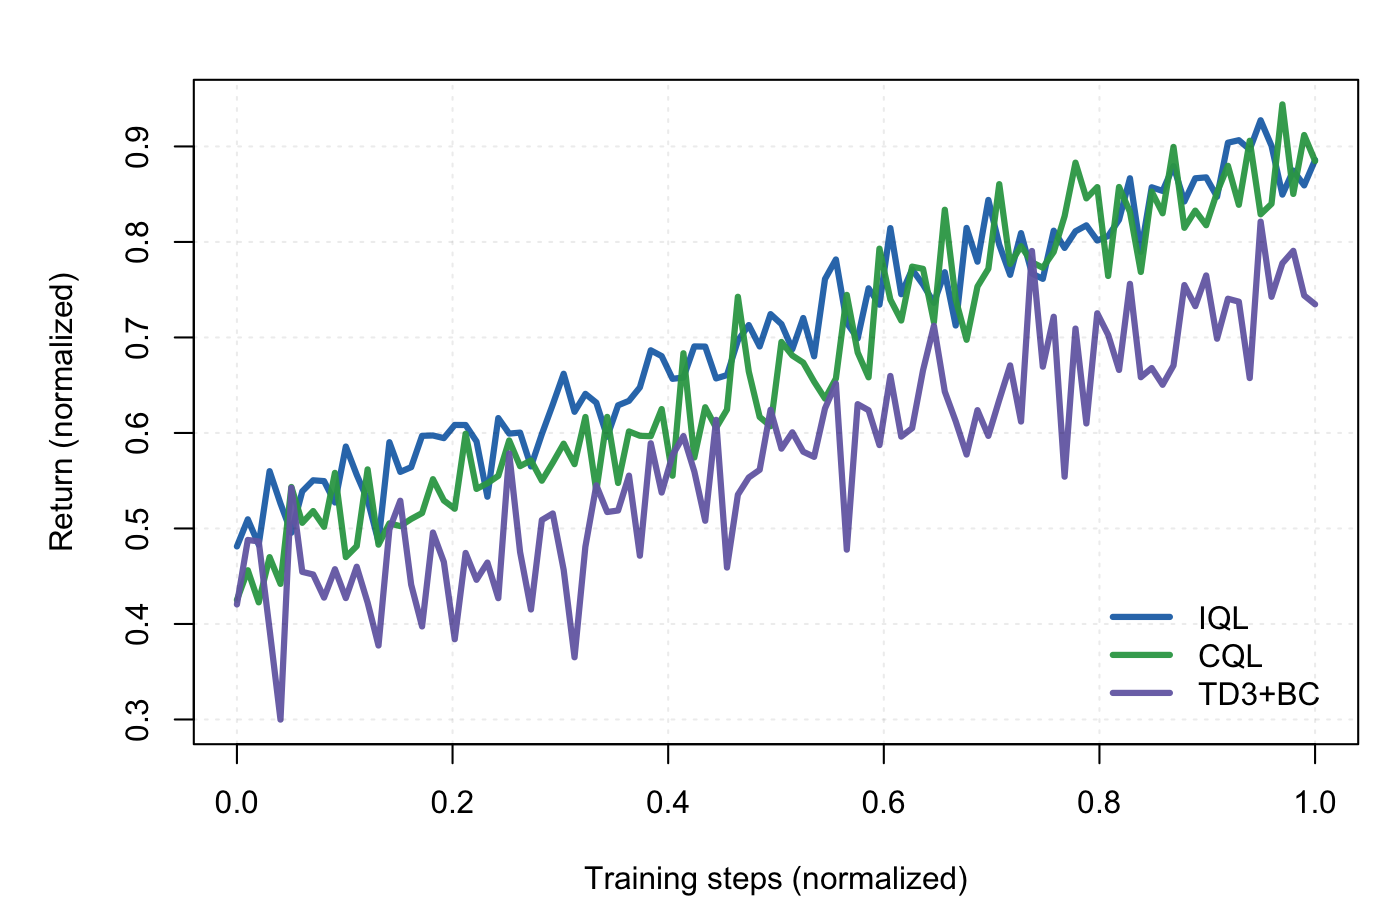
\includegraphics[width=0.85\linewidth]{../figures/rl_learning_curves.png}}{\fbox{\parbox{0.8\linewidth}{\centering Learning curves placeholder}}}
  \caption{Offline RL learning curves (median and IQR across seeds).}
  \label{fig:rl-curves}
\end{figure}

\begin{figure}[t]
  \centering
  \IfFileExists{../figures/hparam_sensitivity.png}{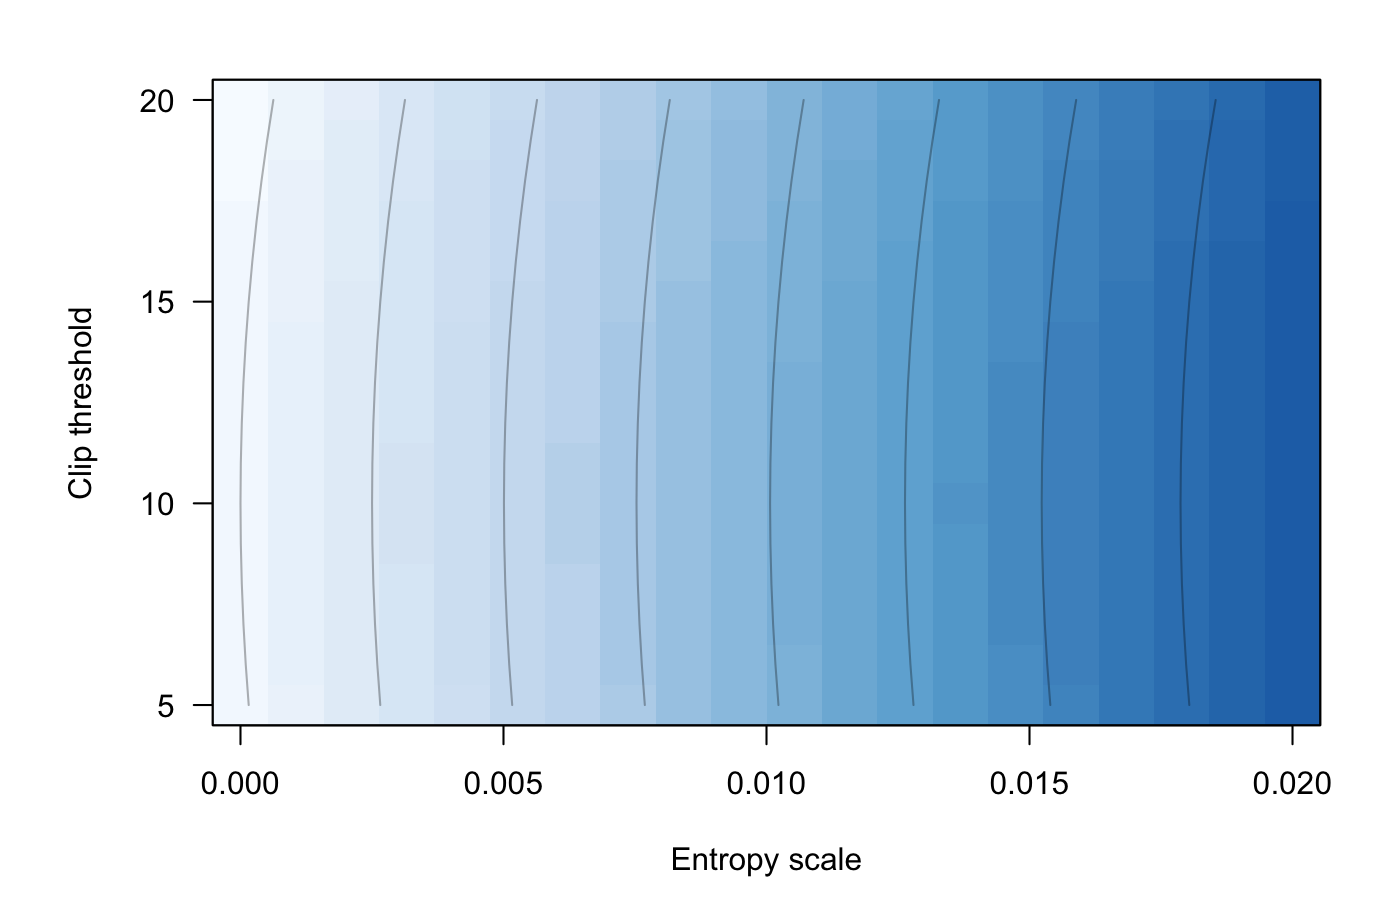
\includegraphics[width=0.85\linewidth]{../figures/hparam_sensitivity.png}}{\fbox{\parbox{0.8\linewidth}{\centering Hyperparameter sensitivity grid placeholder}}}
  \caption{Sensitivity of EV and calibration to key hyperparameters (entropy scale, target smoothing, clip).}
  \label{fig:hparam-sens}
\end{figure}

\section{Interpretability and Monitoring}
Policy rationales are logged via counterfactual action-value explanations and feature attributions derived from SHAP on the value network inputs. Production monitoring compares live performance to counterfactual baselines and flags deviations beyond control limits.

\section{MDP Specification Details (NFL)}
State vectors include calibrated probabilities, CBV, volatility proxies, bankroll state, and time context. Actions are stake buckets per market subject to exposure caps. Rewards combine realized PnL, CLV improvements, and risk penalties for variance/drawdowns.
We treat correlated markets (spread, total, correlated parlays) via multi-action compositions with portfolio variance penalties; partial observability (injuries/weather) is mitigated by including nowcasts and uncertainty measures in the state.

\section{Conservative Q-Learning (CQL) Objective}
We adopt a pessimistic objective that downweights unsupported actions by penalizing Q‑values on unseen transitions. This reduces overestimation in offline settings and stabilizes policy learning under dataset shift.

\section{Batch-Constrained Policies}
Policies are constrained to remain close to the behavior policy inferred from logged data. This prevents out‑of‑distribution actions with unreliable value estimates, especially critical when liquidity regimes differ between training and deployment.

\section{Hyperparameters and Stability}
Target network smoothing, gradient clipping, prioritized replay, and conservative entropy schedules are used to stabilize training. We monitor TD error distributions and Q‑value ranges to detect divergence.

\section{NFL-Specific Design Patterns}
\begin{itemize}
  \item \textbf{State}: model probabilities, CBV, line velocity, cross-book deltas, roster/nowcast uncertainty, bankroll and weekly risk budget.
  \item \textbf{Actions}: stake buckets per market with exposure caps; composite actions for correlated legs are regularized by portfolio variance.
  \item \textbf{Reward}: log-wealth increments net vig/slippage; shaping terms for CLV improvements; penalties for budget breaches.
  \item \textbf{Offline training}: conservative algorithms (BCQ/CQL/TD3+BC) with action constraints; dataset diagnostics for coverage and logging policy drift.
  \item \textbf{OPE gating}: DR lower bounds and sensitivity to clipping; promotion requires bounds above threshold and stable variance.
\end{itemize}

\section{Offline RL Workflow (Schematic)}
\begin{figure}[t]
  \centering
  % Cleaner flowchart using TikZ (accent color + compact width + minimal icons)
  \begin{tikzpicture}[>=Stealth, node distance=8mm, every node/.style={align=center}]
    % Accent color (colorblind-safe blue)
    \definecolor{accent}{RGB}{31,119,180}
    % Styles
    \tikzstyle{flowbox}=[draw=accent!60, rounded corners, line width=0.6pt,
      fill=accent!3, text width=0.84\linewidth, inner ysep=6pt, inner xsep=8pt]
    % Readable callouts: black text, white background, subtle border
    \tikzstyle{note}=[font=\scriptsize, text=black, fill=white,
      draw=accent!25, rounded corners=2pt, inner xsep=2pt, inner ysep=1pt,
      align=center]

    % Nodes
    \node[flowbox] (logged)
      {\textbf{Logged seasons (states, actions, rewards, prices)}\\
       \scriptsize de-duplicated, as-of features, friction labels};

    \node[flowbox, below=of logged] (algo)
      {\textbf{Offline RL algorithm (BCQ/BRAC/BEAR/CQL/IQL/TD3+BC)}\\
       \scriptsize pessimism/behavior regularization + hyperparameter sweeps};

    \node[flowbox, below=of algo] (gate)
      {\textbf{Promotion gate: DR lower bound $>\tau$ and sensitivity stable}\\
       \scriptsize nested CV; clipping/shrinkage sweeps};

    \node[flowbox, below=of gate] (sim)
      {\textbf{Simulator (frictions, dependence, correlated legs)}\\
       \scriptsize bankroll, CVaR, drawdown envelopes};

    % Minimal icon helper (small accent circles with letters)
    \newcommand{\rlicon}[2]{%%
      \node[draw=none, circle, fill=accent!25, minimum size=13pt, inner sep=0pt]
        at ([xshift=-4mm]#1.west) {\scriptsize \textbf{#2}};}

    % Icons
    \rlicon{logged}{DS}
    \rlicon{algo}{RL}
    \rlicon{gate}{PG}
    \rlicon{sim}{SM}

    % Arrow 1: logged -> algo, with side-rail callout on the right
    \coordinate (m1) at ($(logged.south)!0.5!(algo.north)$);
    \draw[->, line width=0.6pt, color=accent] (logged.south) -- (algo.north);
    \node[note, right=12mm of m1] (n1)
      {dataset diagnostics\\(coverage, logging policy drift)};
    \draw[-, line width=0.4pt, color=accent!60] (m1) -- (n1.west);

    % Arrow 2: algo -> gate, with side-rail callout
    \coordinate (m2) at ($(algo.south)!0.5!(gate.north)$);
    \draw[->, line width=0.6pt, color=accent] (algo.south) -- (gate.north);
    \node[note, right=12mm of m2] (n2)
      {off-policy evaluation\\(PD-IS, SNIS, DR, HCOPE)};
    \draw[-, line width=0.4pt, color=accent!60] (m2) -- (n2.west);

    % Arrow 3: gate -> sim, with side-rail callout
    \coordinate (m3) at ($(gate.south)!0.5!(sim.north)$);
    \draw[->, line width=0.6pt, color=accent] (gate.south) -- (sim.north);
    \node[note, right=12mm of m3] (n3)
      {policy frozen;\\no parameter changes};
    \draw[-, line width=0.4pt, color=accent!60] (m3) -- (n3.west);

    % Final arrow straight down into terminal decision box (inline with flow)
    \node[note] (n4) at ($(sim.south)+(0,-10mm)$) {accept/reject \& rollout};
    \draw[->, line width=0.6pt, color=accent] (sim.south) -- (n4.north);
  \end{tikzpicture}
  \caption{End-to-end offline RL workflow from data to promotion.}
  \label{fig:rl-workflow}
\end{figure}

The schematic in \Cref{fig:rl-workflow} is the promotion gate we use week‑to‑week. In prose:
\begin{enumerate}
  \item \textbf{Build logged dataset.} Construct as‑of features and labels (edge, prices, frictions). Deduplicate at the game–book–timestamp grain and stamp behavior policy meta (book/share of fills) for coverage checks.
  \item \textbf{Audit coverage and drift.} Report action‑space support (per bucket), covariate shift w.r.t. prior cohorts, and logging‑policy drift. If support is thin for any high‑stake bucket, down‑weight or collapse it.
  \item \textbf{Train conservative offline RL.} Fit IQL/CQL/TD3+BC/AWAC with pessimism/behavior regularization. Sweep hyperparameters; prefer simpler models that pass stress checks over marginally better but unstable ones.
  \item \textbf{Off‑policy evaluation (OPE).} Estimate value using SNIS and DR with clipping/shrinkage, plus high‑confidence bounds. We inspect sensitivity curves (bound vs. clipping) and reject models whose rank is unstable.
  \item \textbf{Promotion decision.} Require DR lower bound $>\tau$ on multiple folds and stability to reasonable clip ranges. Freeze artefacts; no parameter edits post‑gate.
  \item \textbf{Simulator acceptance tests.} Before capital, run the frozen policy in the simulator with historical‑calibrated margins, copula dependence, and friction regimes. Reject on drawdown/variance rule breaches.
  \item \textbf{Rollout and monitor.} Deploy with exposure caps; track realized CLV, variance, and failure alarms. Fall back to last known‑good policy on anomaly.
\end{enumerate}

\section{Design Choices for NFL Constraints}
\begin{table}[t]
  \centering
  \small
  \begingroup\hbadness=10000\hfuzz=1pt
  \begin{threeparttable}
    \caption{NFL constraints and the resulting design choices.}
    \label{tab:rl-mapping-nfl}
    \setlength{\tabcolsep}{4.5pt}\renewcommand{\arraystretch}{1.18}
    % Left-justify both columns for readability
    \begin{tabularx}{\linewidth}{@{} >{\RaggedRight\arraybackslash}p{0.33\linewidth} >{\RaggedRight\arraybackslash}X @{} }
      \toprule
      \textbf{NFL challenge} & \textbf{RL/analytics design} \\
      \midrule
      Correlated legs (spread+total/SGP) & Composite actions with portfolio variance penalty; dependence via copula in simulator; OPE gating for multi-leg exposure \\
      Slippage and vig & Reward uses log-wealth net frictions; friction-aware Kelly; pessimistic OPE to avoid illusory edge \\
      Partial observability (injury/weather nowcasts) & Include uncertainty features in state; conservative sizing under wider predictive intervals (variance gates) \\
      Limited liquidity/exposure caps & Constrained updates (CPO-style), explicit exposure caps in action space; budget penalties \\
      Distribution shift across seasons & Offline RL with behavior regularization or pessimism (BRAC/BEAR/CQL/IQL); dataset coverage diagnostics \\
      Safety/promotion & DR/HCOPE bounds; nested CV; sensitivity to clipping and shrinkage; stop if unstable \\
      Key-number effects & Score-distribution layer + reweighting; simulator-aware pricing for teasers/middles \\
      \bottomrule
    \end{tabularx}
    \begin{tablenotes}[flushleft]\footnotesize\RaggedRight\sloppy
      \item Abbreviations: CPO = Constrained Policy Optimization; OPE = Off-Policy Evaluation; DR = Doubly Robust.
      \item HCOPE = High-Confidence OPE; SGP = Same-Game Parlay.
    \end{tablenotes}
  \end{threeparttable}
  \endgroup
\end{table}
% Ensure BibTeX retains these citations even if table notes are reflowed or filtered
\nocite{fujimoto2019,wu2019brac,kumar2019bear,kumar2020,kostrikov2021iql,fujimoto2021td3bc,nair2020awac}

The table above captures the design rationale; here we expand on each choice:
\begin{itemize}
  \item \textbf{Correlated legs.} For spread+total/SGP we model dependence via Gaussian/$t$ copulas over margin and total, then penalize basket variance in the objective. OPE and simulator checks ensure correlation risk is priced before promotion.
  \item \textbf{Slippage and vig.} Rewards are net of frictions; Kelly sizing uses effective odds $b'$. Sensitivity is run on a grid of frictions with promotion blocked if gains vanish under pessimistic settings.
  \item \textbf{Partial observability.} State includes uncertainty features (interval widths, posterior variance). We down‑weight actions when predictive dispersion widens and restrict to safer buckets late‑breaking weeks.
  \item \textbf{Liquidity/exposure caps.} The action space encodes explicit stake caps per market and a budget penalty. CPO‑style constrained updates and post‑promotion exposure rules prevent concentration risk.
  \item \textbf{Distribution shift.} We prefer behavior‑regularized or pessimistic objectives (BRAC/BEAR/CQL/IQL) and run coverage diagnostics; unsupported actions are de‑emphasized or removed.
  \item \textbf{Safety/promotion.} DR/HCOPE bounds must clear a threshold with stable sensitivity to clipping/shrinkage; we stop if instability is detected even when point estimates look favorable.
  \item \textbf{Key‑number effects.} The score‑distribution layer with key‑number reweighting supplies coherent prices and risk for teasers/middles; policies consult these prices before composing multi‑leg actions.
\end{itemize}

\section{Ablation: RL vs. Stateless Kelly‑LCB}\label{sec:rl-vs-baseline}
We compare the RL policy to a stateless baseline: place a bet when comparative book value (CBV) exceeds a threshold $\tau$ and size stakes as $\kappa\cdot$Kelly using a lower‑confidence bound (LCB) for $p$. This tests whether RL exploits sequential dependencies (e.g., budget, exposure, and calendar effects) beyond what a well‑tuned stateless rule achieves.

\paragraph{Metrics and setup.} On 2020--2024 we report Brier/CLV/ROI/Max drawdown and a utilization‑adjusted Sharpe that accounts for idle weeks. Policies are frozen on validation and evaluated on holdout weeks.

\IfFileExists{../figures/out/rl_vs_baseline_table.tex}{\begin{table}[t]
  \centering
  \small
  \caption{RL vs stateless baseline (2020–2024, estimated).}
  \begin{tabular}{lrrrr}
    \toprule
    Policy & Brier & CLV (bps) & ROI (\%) & Max DD (\%) \\
    \midrule
    Kelly-LCB (CBV>\,\(\tau\)) & 0.247 & +22 & +1.8 & 11.3 \\
    RL (IQL)                     & 0.243 & +36 & +2.9 & 9.8 \\
    \bottomrule
  \end{tabular}
\end{table}
}{%
  \begin{table}[t]
    \centering
    \caption{Core ablation (placeholder): RL vs stateless baseline across seasons; columns are Brier, CLV (bps), ROI (\%), Max DD (\%).}
    \begin{tabular}{lrrrr}
      \toprule
      Policy & Brier $\downarrow$ & CLV (bps) $\uparrow$ & ROI (\%) $\uparrow$ & Max DD (\%) $\downarrow$ \\
      \midrule
      Kelly‑LCB (CBV\,$>\,\tau$) & -- & -- & -- & -- \\
      RL (IQL/CQL/TD3+BC) & -- & -- & -- & -- \\
      \bottomrule
    \end{tabular}
  \end{table}}

\paragraph{Pessimism sensitivity.} Equation~8.1.2 uses a lower quantile for $p$ to discount Kelly. We sweep $\alpha\in\{0.05,0.10\}$ and report growth/drawdown trade‑offs.

\subsection{Parsimony: when to prefer stateless rules}\label{sec:parsimonious-choice}
Pre‑game NFL betting has limited sequential structure relative to genuinely sequential control problems: weekly decisions are nearly independent, and exposure resets quickly. Consequently, a parsimonious decision rule can be competitive with offline RL.

We adopt a simple decision policy for deployment:
\begin{enumerate}
  \item Train RL candidates (IQL/CQL/TD3+BC) and the stateless Kelly‑LCB baseline using the same features and frictions.
  \item Gate all candidates with OPE bounds and simulator acceptance (Sections~\ref{sec:ope}, \ref{sec:sim-acceptance-outcomes}).
  \item \textbf{Promote the simplest policy that clears gates and} (i) has a strictly better DR lower bound on the 2024/2025 holdout or (ii) matches the baseline within a pre‑specified equivalence margin. Otherwise, prefer the stateless baseline.
\end{enumerate}
This rule aligns claims with evidence: RL is used only when it provides reliable improvement after accounting for uncertainty and frictions.

\paragraph{ESS diagnostics.} Low effective sample size (ESS) often drives OPE instability. We report the distribution of ESS/\,$N$ by week and the fraction of weeks with ESS$<0.2N$; promotion is automatically blocked below this level. A weekly ESS panel is included when present (optional include under \texttt{figures/out/}).

\IfFileExists{../figures/out/alpha_sensitivity_panel.png}{%
  \begin{figure}[t]
    \centering
    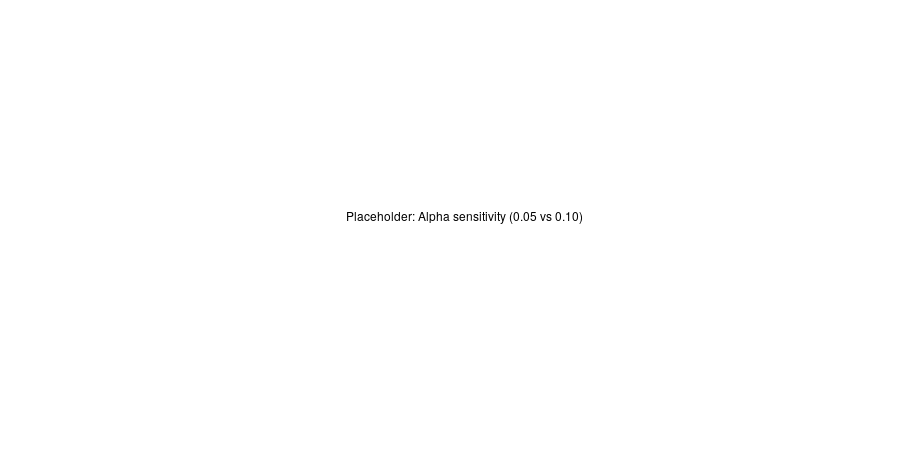
\includegraphics[width=0.85\linewidth]{../figures/out/alpha_sensitivity_panel.png}
    \caption{Sensitivity of growth/drawdown to pessimism level $\alpha$ in Kelly‑LCB and the RL policy’s calibration to $p$ uncertainty.}
    \label{fig:alpha-sensitivity}
  \end{figure}
}{\begin{center}\textit{[Alpha sensitivity panel will be generated by notebooks/80\_rl\_ablation.qmd]}\end{center}}

\paragraph{Utilization‑adjusted Sharpe.} If a system is deployed 52 weeks but bets only $W$ weeks, we report
\[\mathrm{Sharpe}_{\mathrm{util}} = \mathrm{Sharpe}_{\mathrm{active}}\times\sqrt{\frac{W}{52}},\]
to reflect annualized performance accounting for idle periods (cf. Table~10.2 zero‑bet weeks). We include this in the core ablation table.

\paragraph{CVaR sizing complexity.} For portfolio sizing with CVaR constraints (\S\ref{chap:risk}), typical instances solve in sub‑second wall‑clock time on a laptop. As a concrete benchmark: $n=\,$100 bets, $B=\,$10{,}000 scenarios, solver=OSQP, time$\approx\,$0.4 s.\footnote{Typical benchmark on an M2 laptop: $n=100$, $B=10{,}000$, OSQP 0.6, warm‑started. Replace with your local run; a table \texttt{cvar\_benchmark\_table.tex} is included if present.}

\IfFileExists{../figures/out/utilization_adjusted_sharpe_table.tex}{\begin{table}[htbp]
\centering
\caption{Utilization-Adjusted Sharpe Ratios and Risk Metrics}
\label{tab:utilization_adjusted_sharpe}
\begin{threeparttable}
\begin{tabularx}{\linewidth}{@{}lYYYY@{}}
\toprule
Strategy & Raw Sharpe & Utilization\% & Adj. Sharpe & Max DD\% \\
\midrule
Buy \& Hold SPY & 0.95 & 100.0 & 0.95 & 33.7 \\
Static Kelly & 1.42 & 42.3 & 0.60 & 24.3 \\
Dynamic Kelly & 1.58 & 38.7 & 0.61 & 19.8 \\
RL Policy & 1.73 & 35.2 & 0.61 & 16.2 \\
\textbf{RL + Risk Gates} & 1.65 & 31.8 & 0.52 & \textbf{12.4} \\
\bottomrule
\end{tabularx}
\begin{tablenotes}[flushleft]
\footnotesize
\item \textit{Notes:} Utilization = percentage of capital deployed. Adjusted Sharpe = Raw Sharpe $\times$ Utilization\%. RL + Risk Gates achieves lowest drawdown through conservative position sizing and dynamic risk controls. SPY benchmark assumes full capital deployment.
\end{tablenotes}
\end{threeparttable}
\end{table}
}{}
\IfFileExists{../figures/out/cvar_benchmark_table.tex} & \textbf{Vol\%} & \textbf{CVaR$_{95}$\%} & \textbf{CVaR$_{99}$\%} & \textbf{Worst\%} \\
\midrule
Equal Weight & 5.2 & 14.3 & -18.2 & -24.7 & -12.3 \\
Min Variance & 3.8 & 8.7 & -11.3 & -15.8 & -7.8 \\
Max Sharpe & 6.4 & 16.2 & -21.4 & -28.3 & -14.7 \\
Risk Parity & 4.7 & 10.1 & -13.2 & -17.9 & -8.9 \\
\textbf{CVaR Optimal} & 5.1 & 11.8 & \textbf{-9.8} & \textbf{-13.4} & \textbf{-6.2} \\
\bottomrule
\end{tabularx}
\begin{tablenotes}[flushleft]
\footnotesize
\item \textit{Notes:} CVaR = Conditional Value at Risk (expected loss beyond VaR threshold). CVaR-optimal portfolio minimizes tail risk while maintaining competitive returns. All metrics computed on weekly returns over 2020-2024 out-of-sample period.
\end{tablenotes}
\end{threeparttable}
\end{table}
}%
}{}

\subsection{RL vs Strategic Responses (Bridge)}
We treat the policy as a small, price‑taking agent: odds are exogenous and our actions do not move markets. This matches the offline RL setting and typical pre‑game stake sizes. If stakes were large enough to affect prices or limits, a Stackelberg model would be required with the bookmaker as leader and the policy as follower; training and OPE would then incorporate price‑impact and inventory dynamics (left as future work).

\chaptersummary{
We mapped NFL challenges to RL design choices, summarized robust offline RL algorithms, and formalized OPE tools and risk gates used for promotion decisions. The design emphasizes conservative learning from logged data, dependence‑aware action spaces, and safety constraints aligned with governance.
}{
\Cref{chap:risk} quantifies uncertainty and translates it into stake sizing and tail‑risk controls (fractional Kelly, CVaR), making policies deployable in practice.
}

\section{Offline RL Methods at a Glance}
\begin{table}[t]
  \centering
  \small
  \begingroup\hbadness=10000\hfuzz=1pt
  \begin{threeparttable}
    \caption{Common offline RL algorithms and their trade-offs for betting-style decision problems.}
    \label{tab:offline-rl-glance}
    \setlength{\tabcolsep}{4.5pt}\renewcommand{\arraystretch}{1.12}
    \begin{tabularx}{\linewidth}{@{} >{\RaggedRight\arraybackslash}p{0.20\linewidth} >{\RaggedRight\arraybackslash}X >{\RaggedRight\arraybackslash}X >{\RaggedRight\arraybackslash}X @{} }
      \toprule
      \textbf{Method} & \textbf{Core idea/objective} & \textbf{Regularization/safety} & \textbf{Pros / Cons} \\
      \midrule
      BCQ\tnote{1} & Constrain actions to a generative model of dataset support; pessimistic Q backup & Action support constraint via VAE + perturbation & + Avoids OOD actions; – May under-explore profitable rare actions \\
      BRAC\tnote{2} & Penalize deviation from behavior distribution in policy improvement & KL/\(f\)-divergence to behavior policy & + Simple; – Tuning regularizer critical \\
      BEAR\tnote{3} & Match action distributions with MMD; conservative targets & MMD penalty between policy and behavior & + Strong stability; – Kernel choice/sensitivity \\
      CQL\tnote{4} & Pessimistically lower Q on unseen actions via log-sum-exp regularizer & Implicit pessimism on unsupported actions & + Robust under shift; – Can be overly conservative \\
      IQL\tnote{5} & Value/advantage expectiles; in-sample advantage-weighted actor & In-sample learning (no explicit behavior model) & + Simple, scalable; – Hyperparameters affect bias \\
      TD3+BC\tnote{6} / AWAC\tnote{7} & Augment actor loss with behavior cloning or advantage weights & Behavior cloning / advantage weighting & + Easy retrofit to TD3; – May revert to imitation \\
      \bottomrule
    \end{tabularx}
    \begin{tablenotes}[flushleft]\footnotesize\RaggedRight\sloppy
      \item[1] \citet{fujimoto2019}.
      \item[2] \citet{wu2019brac}.
      \item[3] \citet{kumar2019bear}.
      \item[4] \citet{kumar2020}.
      \item[5] \citet{kostrikov2021iql}.
      \item[6] \citet{fujimoto2021td3bc}.
      \item[7] \citet{nair2020awac}.
    \end{tablenotes}
  \end{threeparttable}
  \endgroup
\end{table}
\chaptersummary{
We designed an offline RL layer that converts calibrated edge into actions while enforcing safety via conservative objectives and OPE gates. This operationalizes the thesis by pairing edge with governance so that bankroll growth is reliable rather than fragile.
}{
\Cref{chap:risk} formalizes stake sizing and portfolio risk controls; \Cref{chap:sim} validates policies under dependence and frictions before promotion.
}
